\documentclass[11pt, a4paper]{article}
\usepackage[utf8]{inputenc}
\usepackage{geometry}
\geometry{margin=1in}
\usepackage{graphicx}
\usepackage{amsmath}
\usepackage{amssymb}
\usepackage{booktabs}
\usepackage{hyperref}
\usepackage{parskip}
\usepackage{caption}
\usepackage{float}
\usepackage{enumitem}
\usepackage{xcolor}

% figures live one level up, in student_plots/ and bipartite_plots/
\graphicspath{{../}}

\hypersetup{colorlinks=true, linkcolor=blue!70!black, urlcolor=blue!70!black}
\captionsetup{font=small}

\title{\textbf{Assignment 1: Opinion Network Formation}\\[0.3em]
\large Three Views of One Survey: Student--Student, Student--Question and Question--Question Networks}
\author{Team \textbf{MATlab matlab?}\\[0.4em] Mayank Kar \quad Tanush Garg \quad Amish Goyal\\ IIIT Hyderabad --- Dynamical Processes on Complex Networks}
\date{September 2026}

\begin{document}
\maketitle

\section{Team Name}
\textbf{MATlab matlab?}

\section{GitHub Repository}
\url{https://github.com/its-amish/DPCN_ass1}

The repository is organised by network: \texttt{Student Network/} (Network~A), \texttt{Extreme Bipartite
Network/} (Networks~B and~C, plus interactive D3 visualisers), and \texttt{Question Network/} (Network~D). The
shared cleaning module \texttt{clean.py} sits at the repository root and is used by Networks~A and~D. Every
figure and number in this report is produced by the notebook in the corresponding folder; the numbers quoted for
Networks~B, C and~D were additionally re-derived from the raw CSV as a cross-check. This report is built from
\texttt{report/report.tex}.

\section{Dataset Documentation}

The survey collects opinions on 60 statements, in four sections of 15: \textbf{T} Technology, \textbf{E} Education,
\textbf{S} Society \& Ethics, \textbf{V} Environment. There are \textbf{96 responses}, each answer on a five-point
Likert scale, giving at most 5{,}760 data points.

\subsection{What the raw answers look like}

\begin{center}
\begin{tabular}{lrr}
\toprule
\textbf{Answer} & \textbf{Count} & \textbf{Share of given answers} \\
\midrule
Strongly Agree & 2{,}251 & 43.1\% \\
Agree & 1{,}914 & 36.7\% \\
Neutral & 686 & 13.1\% \\
Disagree & 256 & 4.9\% \\
Strongly Disagree & 111 & 2.1\% \\
\midrule
Blank & 505 & --- \\
``No Comments'' & 37 & --- \\
\bottomrule
\end{tabular}
\end{center}

Two features of this table drive every decision below. First, the class is
\textbf{overwhelmingly agreeable}: 79.8\% of all given answers are Agree or Strongly Agree and only 7.0\% are any
kind of disagreement. Second, \textbf{missing answers are not scattered}, they arrive in whole sections:

\begin{itemize}[nosep]
  \item 5 respondents (IDs 44, 60, 68, 73, 78) answered \textbf{nothing at all};
  \item 4 respondents (IDs 30, 39, 77, 87) answered \textbf{only the Technology section};
  \item ID 79 skipped all of Environment and ID 123 skipped 10 of its 15 questions;
  \item every other respondent left at most 4 answers blank.
\end{itemize}

Blank cells and the 37 ``No Comments'' answers are treated as missing throughout.

\subsection{Two preparations of the same data}

The three networks need different things from the data, so the project uses two documented preparations.

\begin{center}
\small
\begin{tabular}{p{3.9cm} p{5.2cm} p{5.2cm}}
\toprule
 & \textbf{Preparation 1 (Networks A, D)} & \textbf{Preparation 2 (Networks B, C)} \\
\midrule
Encoding & $-2$ Strongly Disagree \dots $+2$ Strongly Agree; sign = polarity, size = strength
        & $1$ Strongly Disagree \dots $5$ Strongly Agree \\
Respondents removed & only the 5 completely empty responses $\rightarrow$ \textbf{91 students}
        & respondents with no extreme answer $\rightarrow$ \textbf{89 students} \\
Missing answers & kept as missing; each pair of students is compared only on questions \emph{both} answered
        & dropped from the long-format edge list \\
Answers used & all five levels & only Strongly Disagree and Strongly Agree ($\{1,5\}$) \\
Result & 91 students $\times$ 60 questions, 242 missing cells & 2{,}362 extreme responses \\
\bottomrule
\end{tabular}
\end{center}

Preparation~1 is implemented once in \texttt{clean.py}, is shared by Networks~A and~D, and adds 3 to recover the
conventional 1--5 scale, so the two encodings are interchangeable. One caveat should be recorded honestly: the 7 respondents that
Preparation~2 drops for having ``no extreme view'' are mostly not opinion-moderates. Five of them submitted an
empty form and one (ID 77) answered only Technology; \textbf{ID 119 is the only respondent who genuinely
answered the survey without ever using an extreme}. Preparation~2's remaining 89 students therefore still
include three respondents (IDs 30, 39, 87) who answered only 15 of the 60 questions, and their node degrees in
Networks~B and~C are correspondingly understated.

\section{Pipeline Followed}

We build four networks from the same survey, each answering a different question. Two look at the students,
two at the questions, and the two question networks are built on deliberately different definitions of a link.

\begin{center}
\footnotesize
\begin{tabular}{p{1.9cm}p{2.9cm}p{3.2cm}p{2.7cm}p{2.9cm}}
\toprule
 & \textbf{Network A} & \textbf{Network B} & \textbf{Network C} & \textbf{Network D} \\
\midrule
Nodes & 91 students & 89 students + 60 questions & 60 questions & 60 questions \\
Edge means & ``agree more than chance'' & ``holds an extreme view on'' & ``co-held extreme views'' & ``answers rise and fall together'' \\
Type & weighted, one-mode & bipartite, unweighted & weighted projection of B & weighted, thresholded \\
Edges & 2{,}026 & 2{,}362 & 1{,}770 ($K_{60}$) & 188 \\
Author & Mayank Kar & Tanush Garg & Tanush Garg & Amish Goyal \\
\bottomrule
\end{tabular}
\end{center}

Networks~C and~D are both question--question networks, but they are not competing answers to the same question.
C asks \emph{which questions provoke intense feeling in the same students}, and counts only extreme answers; D
asks \emph{which questions move together across the full five-point scale}, and uses every answer. Read together
they separate intensity from alignment.

\subsection{Network A --- student--student agreement}

\textbf{Step 1: a simple agreement score.} For every question both students answered, the pair scores 2 for an
identical answer (including both Neutral), 1 for different answers on the same side of the scale
(Agree/Strongly Agree, or Disagree/Strongly Disagree), and 0 otherwise. Averaging over the $n_{ij}$ questions
both answered and halving gives a score in $[0,1]$:
$$w^{\text{simple}}_{ij} = \frac{1}{2\,n_{ij}} \sum_{q \in \text{shared}} s_q(i,j).$$
Averaging rather than summing matters because the Technology-only students share just 15 questions with
everyone else.

\textbf{Step 2: adjusting for chance.} The simple score never reaches 0 (its minimum over 4{,}095 pairs is
0.133), so a network built from it links \emph{every} student to every other. The cause is the answer
distribution above: when four in five answers are on the agree side, two students drawn at random already match
most of the time. We therefore subtract, for each question, the average score $E_q$ over \emph{all} pairs of
classmates --- what two randomly chosen students would score on that question:
$$w_{ij} = \frac{1}{n_{ij}} \sum_{q \in \text{shared}} \bigl(s_q(i,j) - E_q\bigr).$$
A positive weight now means ``this pair agrees more than two random classmates would''. Matching on a question
the whole class agrees on adds almost nothing; matching on a question that splits the class counts heavily.
\textbf{Network A links every pair with $w_{ij} > 0$}: 2{,}026 edges, 49.5\% of all pairs, one student isolated.

\textbf{Step 3: sparsification.} At 49.5\% density the network is unreadable and its path lengths are
uninformative, so we thin it two ways: a global cutoff swept from weak to strong (experiment 1), and keeping
each student's \textbf{two strongest edges} (experiment 2), which yields a 155-edge network used for drawing and
for the sparse half of the measurements.

\subsection{Network B --- student--question extremes (bipartite)}

Responses are melted into $(\texttt{student}, \texttt{question}, \texttt{response})$ triples and filtered to
$r \in \{1,5\}$, so an edge exists exactly when a student holds an \emph{extreme} view on a question. Moderate
and neutral answers are deliberately discarded: the aim is to map ideological intensity rather than consensus.
The result is a verified bipartite graph $G = (U,V,E)$ with $|U| = 89$, $|V| = 60$, $|E| = 2{,}362$, bipartite
density $0.4423$, and a single connected component.

\subsection{Network C --- question--question projection}

Network B is projected onto the question set:
$$e_{q_i,q_j} \in E_Q \iff \exists\, u \in U : (u,q_i) \in E \wedge (u,q_j) \in E,$$
i.e.\ two questions are linked when at least one student holds extreme views on both. The unweighted projection
turns out to be the complete graph $K_{60}$, so all further analysis uses the \textbf{weighted} projection
$G_Q^W$, where $w_{ij}$ counts the students who hold extreme views on both questions.

\subsection{Network D --- question--question correlation}

Network~D starts from Preparation~1 (the same 91 students and the same $-2 \dots +2$ encoding as Network~A) and
asks, for each of the $\binom{60}{2} = 1{,}770$ question pairs, whether the two statements are answered in step.
The measure is the \textbf{Spearman rank correlation} $\rho_{ij}$, computed over the students who answered both.
Spearman rather than Pearson because Likert answers are ordinal, so only the monotonic relationship is
meaningful.

A correlation matrix is fully connected, so a cutoff is applied: an edge exists iff
$$\rho_{ij} > 0.35,$$
with weight $w_{ij} = \rho_{ij}$ and, for path-based measures, distance $d_{ij} = 1/\rho_{ij}$, so that strongly
correlated statements lie close together. The cutoff discards weak and ambient associations and keeps
moderate-to-strong ones. Eigenvector centrality then identifies the statements at the core of the belief
structure and weighted betweenness the statements bridging otherwise separate groups. Two further tools
describe the grouping. \textbf{Louvain} searches for a split of the questions that maximises modularity, the
share of edge weight falling inside groups minus the share expected if the same edges were rewired at random;
it is used here only to describe the clusters, not to make a claim about their strength. The \textbf{attribute
assortativity coefficient} $r$ is the correlation between the section labels (T, E, S, V) at the two ends of an
edge: $r = 1$ would mean questions link only within their own section, $r = 0$ that the sections say nothing
about which questions link.

\section{Analysis and Visualizations}

\subsection{Network A: student--student agreement}

\textit{Code and figures: \texttt{Student Network/student\_network.ipynb} (Mayank Kar).}

\begin{figure}[H]
\centering
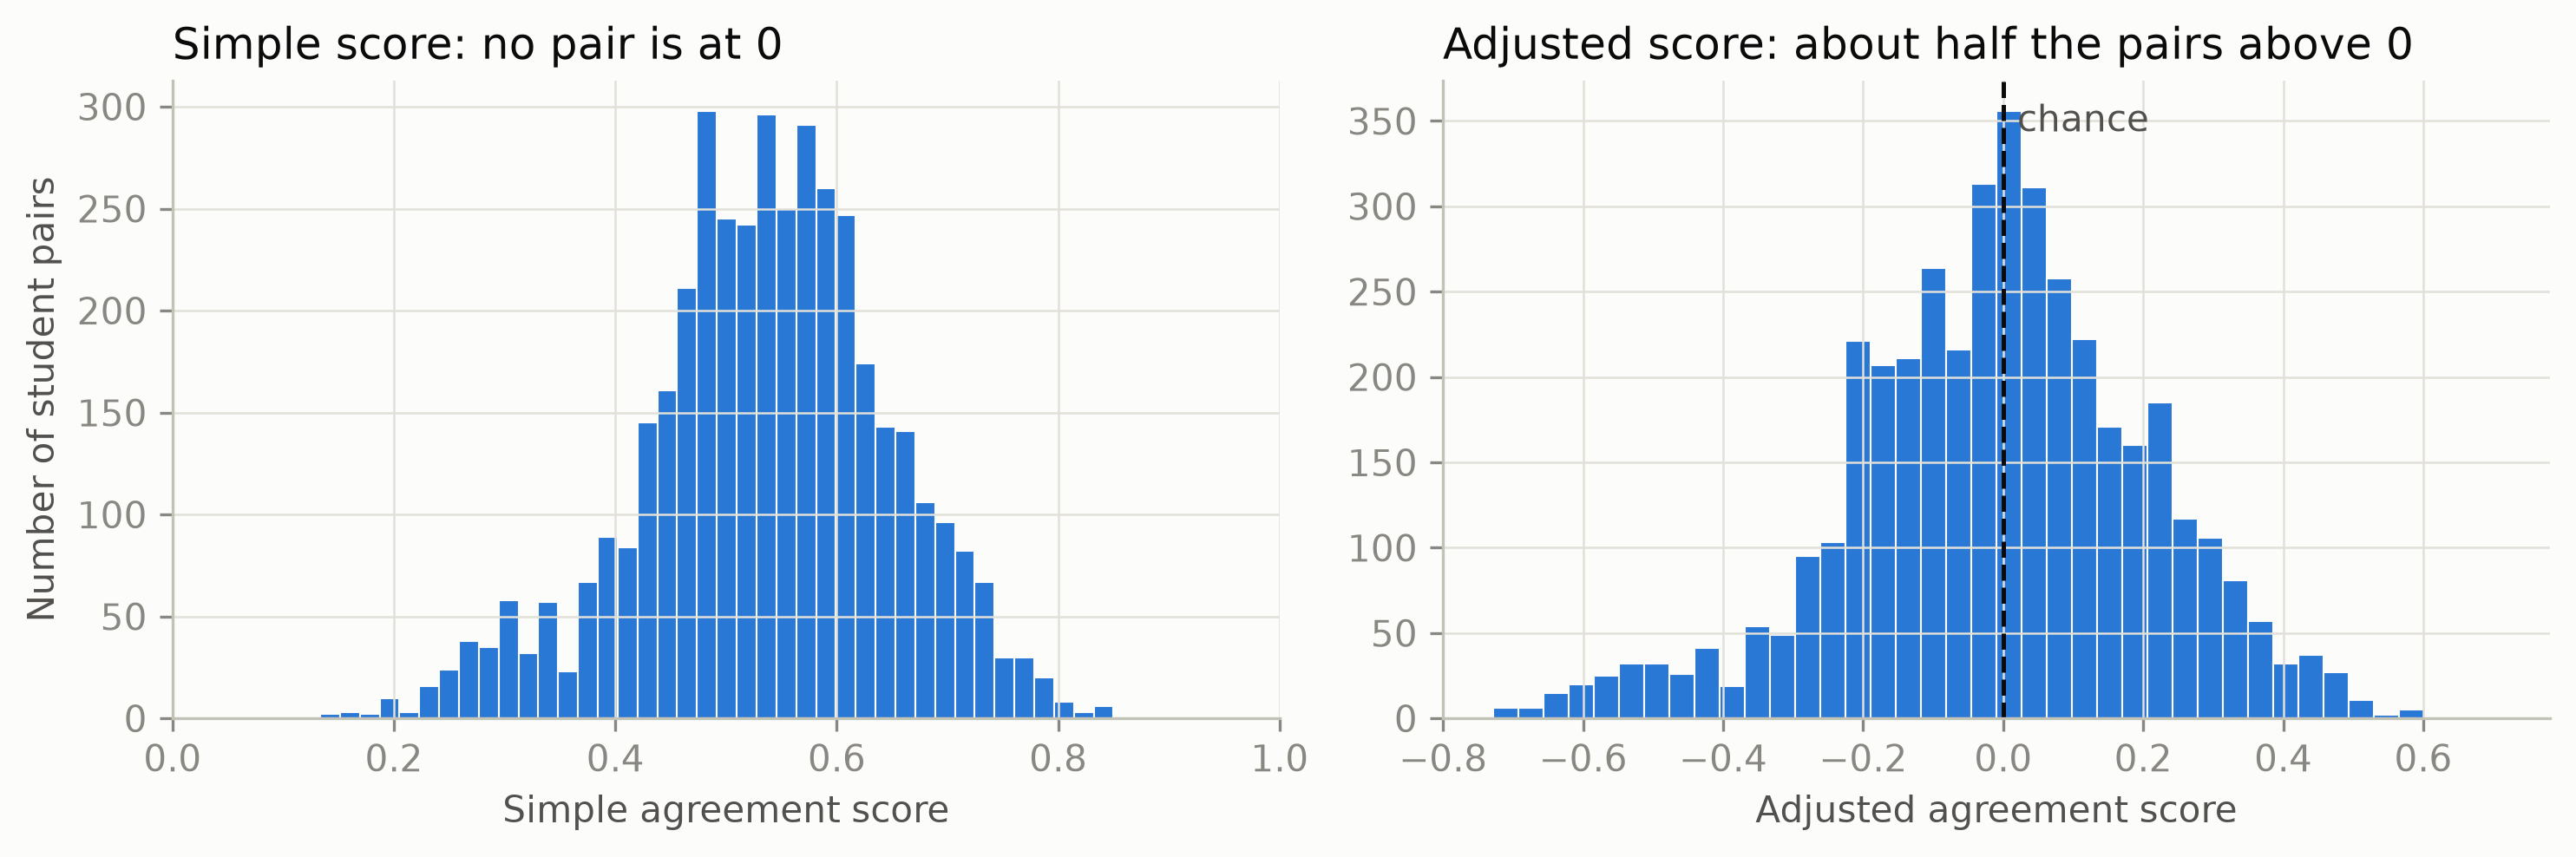
\includegraphics[width=\textwidth]{student_plots/weight_distributions.png}
\caption{Left: the simple agreement score over all 4{,}095 pairs --- no pair sits at 0, so this score cannot
define a network. Right: after subtracting chance agreement the scores centre on 0, and ``above chance''
becomes a meaningful cutoff. 49.5\% of pairs survive it.}
\end{figure}

\begin{figure}[H]
\centering
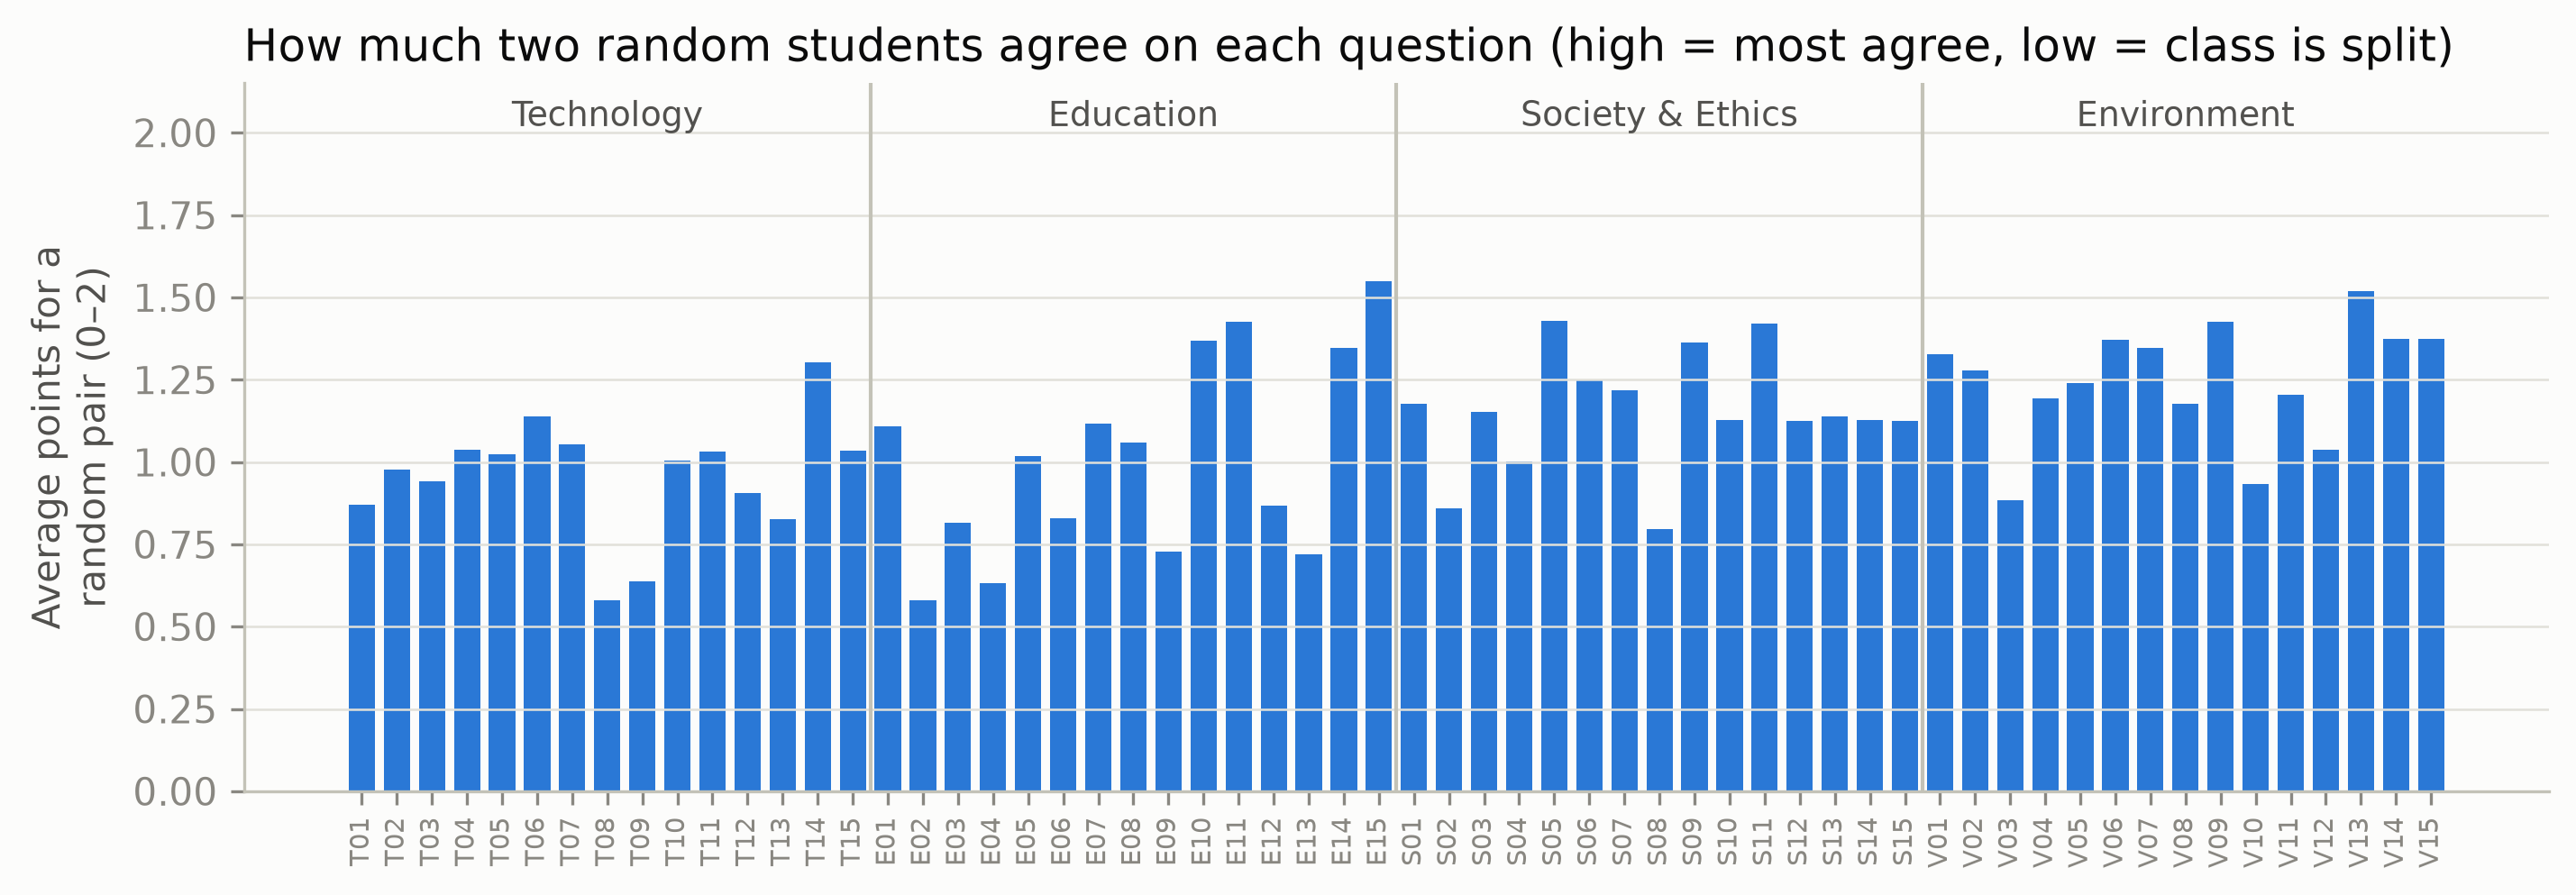
\includegraphics[width=\textwidth]{student_plots/expected_score_per_question.png}
\caption{Chance agreement $E_q$ per question. High bars are consensus questions, where matching answers say
little about a pair; low bars are the questions that actually separate students. The most divisive are E02
(written exams measure knowledge, $E_q = 0.58$), T08 (AI diagnosis, 0.58), E04 (online learning, 0.63) and T09
(autonomous vehicles, 0.64); the most consensual are E15 (1.55), V13 (1.52), S05, E11 and V09 (1.43).}
\end{figure}

\begin{figure}[H]
\centering
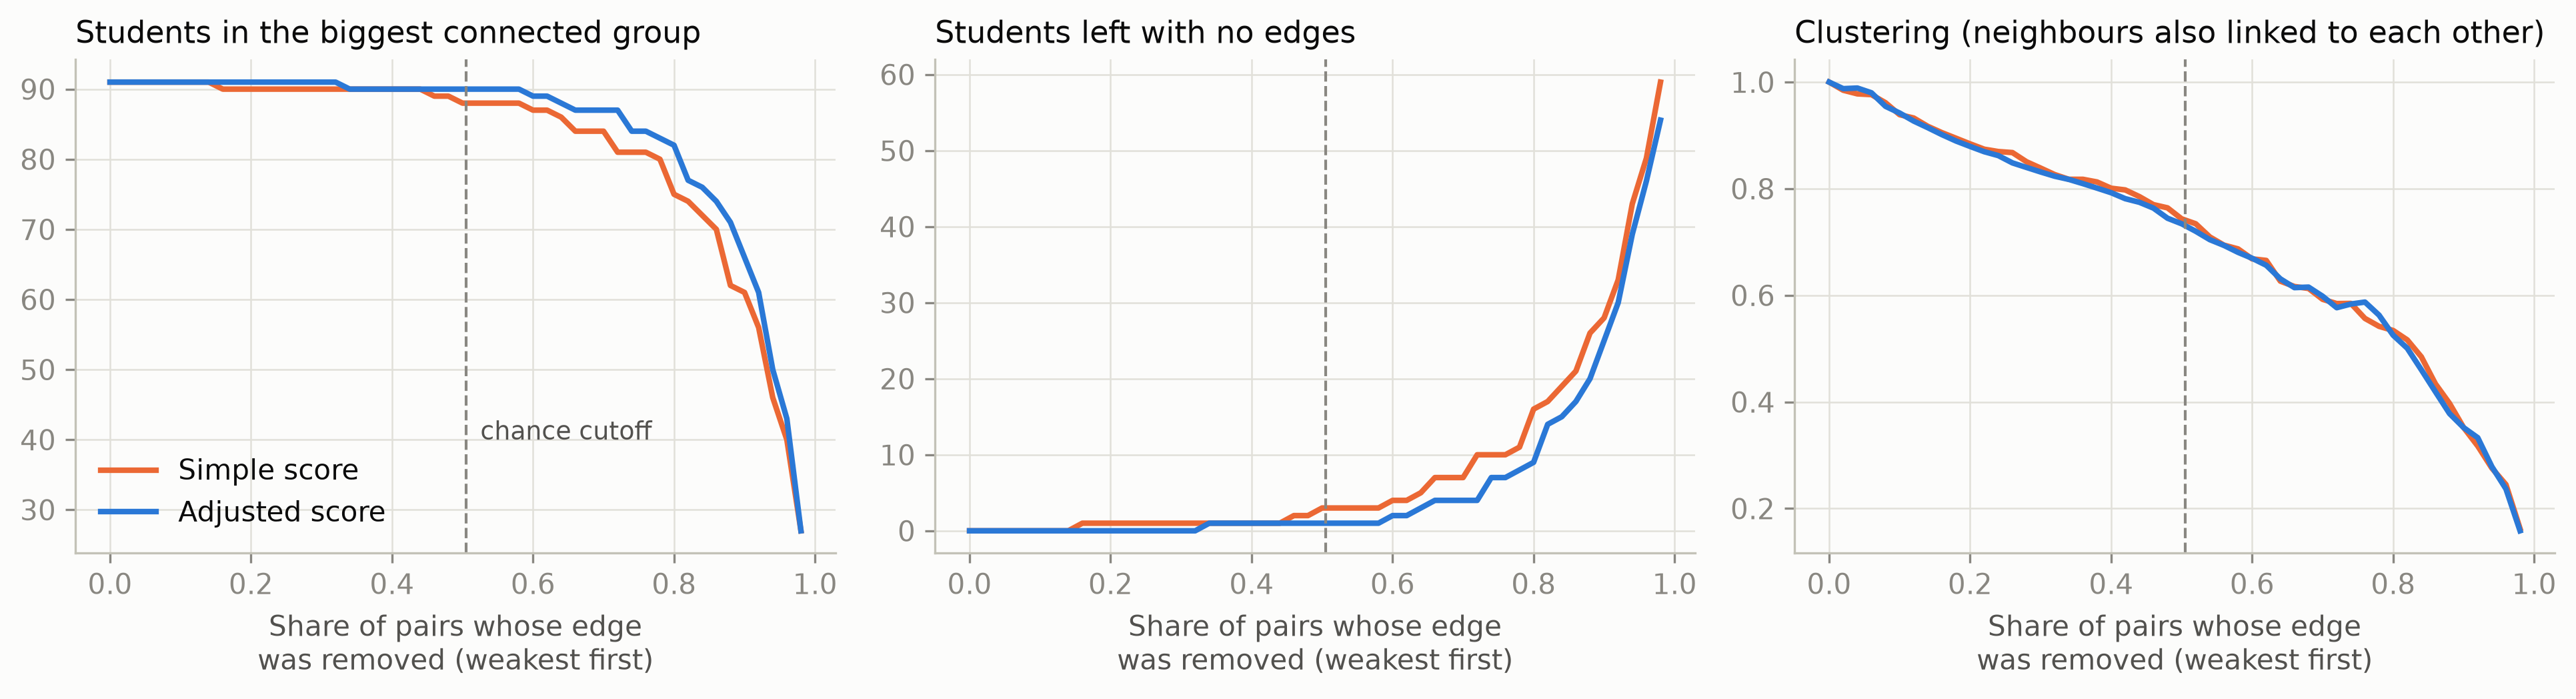
\includegraphics[width=\textwidth]{student_plots/threshold_sweep.png}
\caption{Removing the weakest edges step by step, comparing the simple and adjusted scores at equal density.
The biggest connected group erodes gradually --- there is no percolation-style collapse. The first students cut
off are 120 (no above-chance edge at all), 89, 63 and 22, most of whom answer well below the class average of
$+1.14$. Beyond about 90\% removed the curves describe an empty network rather than the class.}
\end{figure}

\begin{figure}[H]
\centering
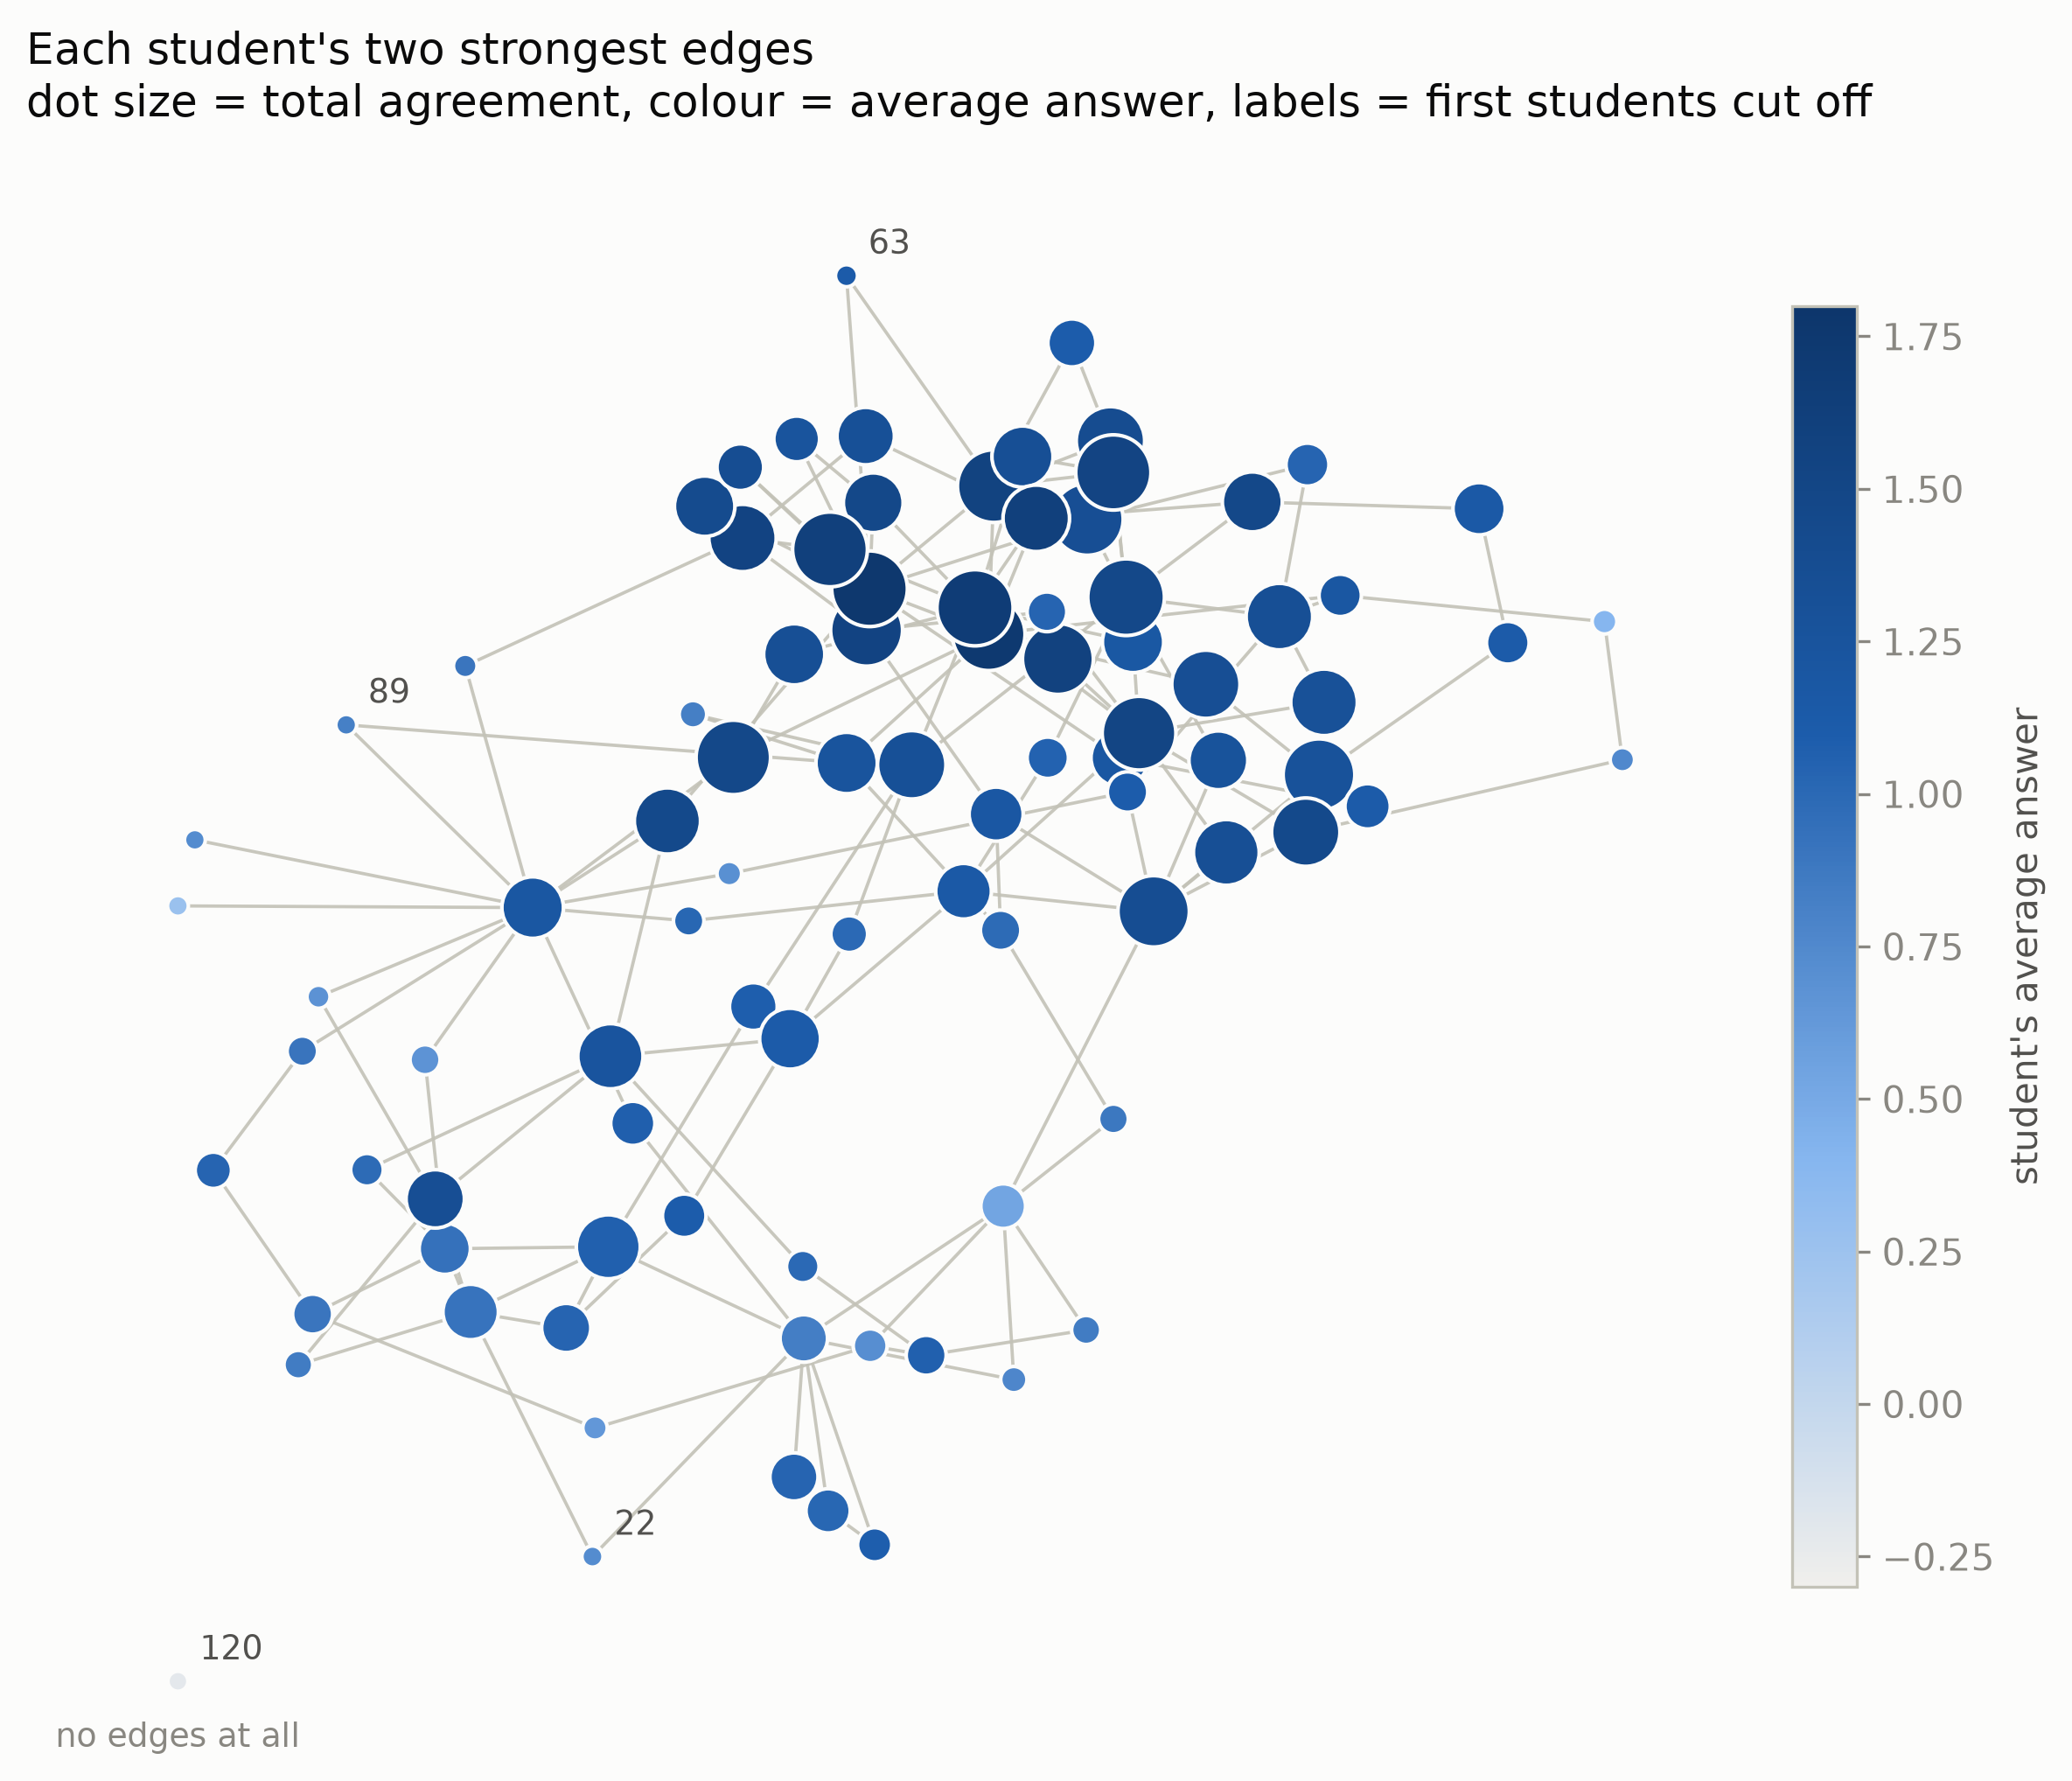
\includegraphics[width=0.92\textwidth]{student_plots/network_drawing.png}
\caption{The network reduced to each student's two strongest edges (155 edges, 3.8\% of pairs). 90 of the 91
students remain in one piece. Dot size is total agreement (strength) in the full network and colour is the
student's average answer: the dark, emphatic answerers form the dense upper core, lighter and more hesitant
students sit on the rim, and student 120 has no edge at all.}
\end{figure}

\begin{figure}[H]
\centering
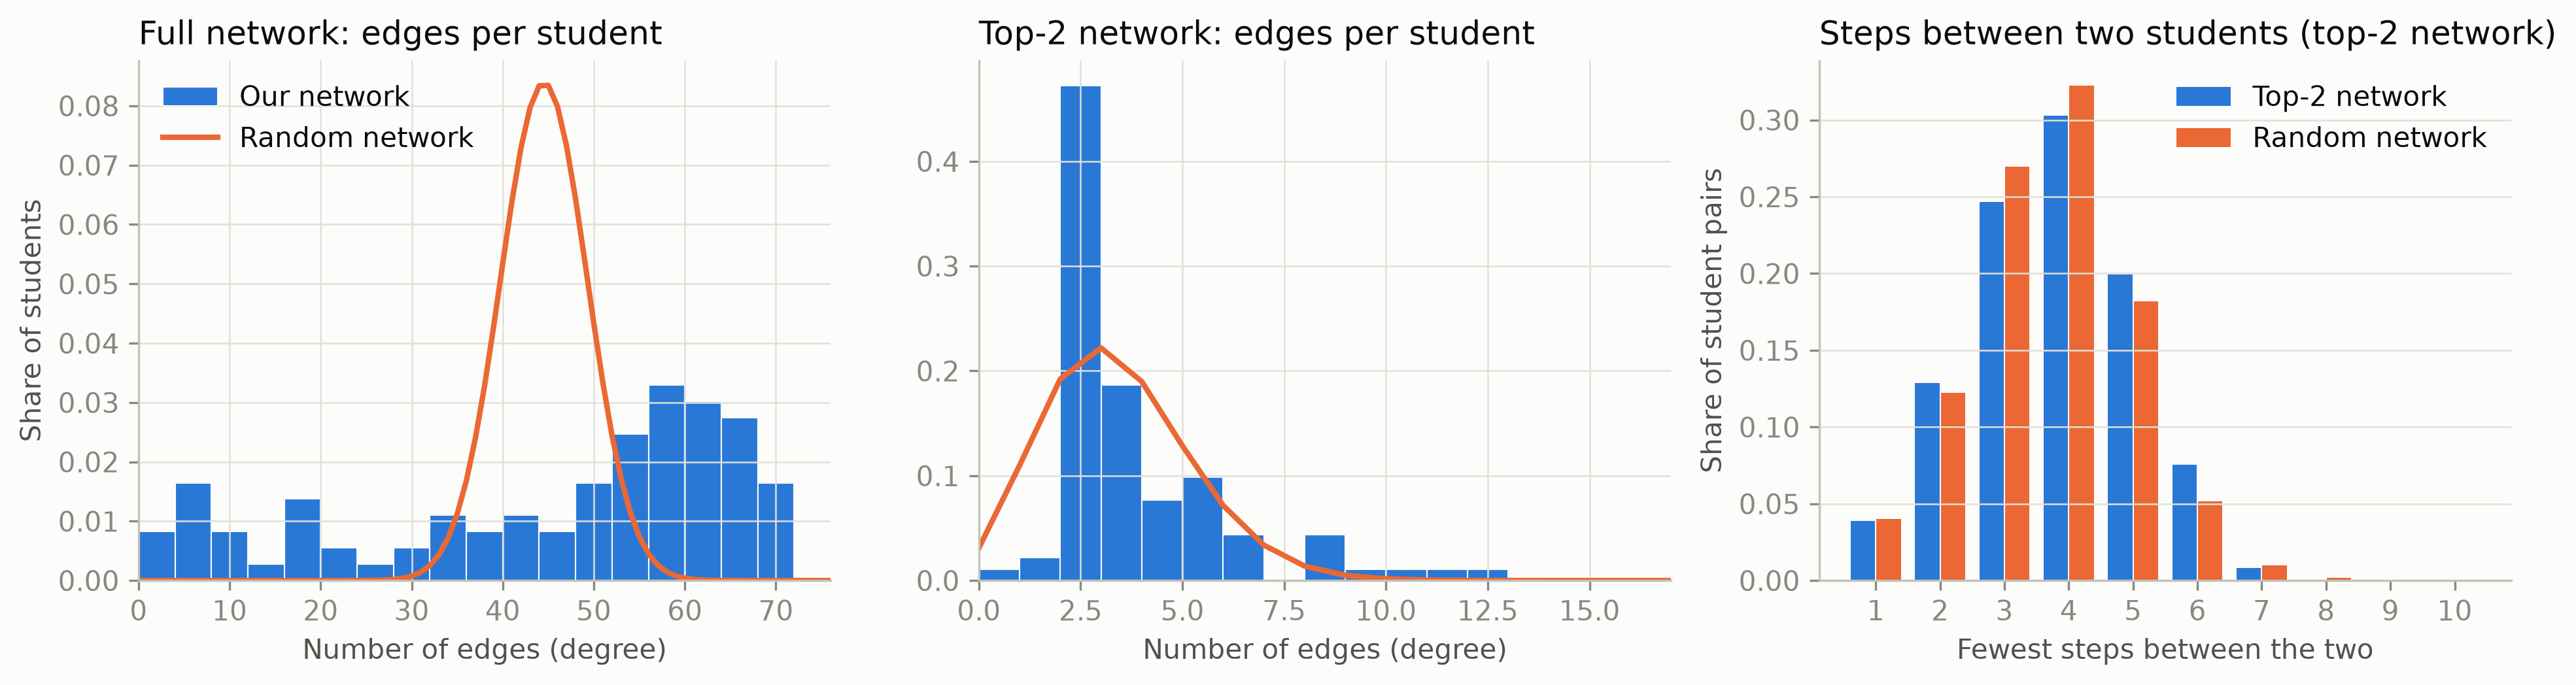
\includegraphics[width=\textwidth]{student_plots/degree_and_path_length.png}
\caption{Left and centre: number of edges per student in the full and top-2 networks, against the binomial
curve of an ER graph of the same size. Both are far broader than random. Right: distances in the top-2 network
are essentially the random values, so the network is short-pathed without being random.}
\end{figure}

\begin{center}
\begin{tabular}{lrrrr}
\toprule
& \textbf{Full network} & \textbf{ER graph} & \textbf{Top-2 network} & \textbf{ER graph} \\
\midrule
Edges & 2{,}026 & 2{,}026 & 155 & 155 \\
Density & 0.495 & 0.495 & 0.038 & 0.038 \\
Mean degree & 44.53 & 44.53 & 3.41 & 3.41 \\
Degree spread ($\sigma_k$) & 21.00 & 4.59 & 2.23 & 1.80 \\
Average clustering & 0.730 & 0.494 & 0.154 & 0.026 \\
Transitivity & 0.757 & 0.494 & 0.090 & --- \\
Average shortest path & 1.52 & 1.51 & 3.76 & 3.65 \\
Diameter & 4 & 2 & 7 & $\approx 5$ \\
Global efficiency & 0.732 & 0.747 & 0.308 & 0.338 \\
Largest component & 90 & 91 & 90 & 87.6 \\
Small-world $\sigma$ & \textbf{1.46} & --- & \textbf{5.66} & --- \\
Degree assortativity & 0.027 & $-0.023$ & $-0.323$ & $-0.023$ \\
\bottomrule
\end{tabular}
\captionof{table}{Network A against ER graphs with the same number of nodes and edges (each ER column is the
mean over 20 such graphs).}
\end{center}

\textbf{Reading the measurements.} Clustering is far above random in both versions --- six times random in the
top-2 network, where each student contributed only two edges --- while distances match the random values. That
is the small-world signature, $\sigma = 1.46$ in the full network and $5.66$ in the sparse one. Degrees are much
more spread out than an ER graph allows (21.0 against 4.6), but bounded: with 91 students there is no evidence
of a power-law. The negative assortativity of the top-2 network is largely constructed, since students naming
the same popular classmate leave that classmate ringed by low-degree neighbours.

Five centrality measures are used, each capturing a different sense of being well placed in the network. They
are defined here once and reused for the question networks in Sections~5.3 and~5.4.

\begin{center}
\small
\begin{tabular}{p{2.6cm} p{5.0cm} p{6.6cm}}
\toprule
\textbf{Measure} & \textbf{Definition} & \textbf{Meaning in Network A} \\
\midrule
Degree & $k_i$, the number of edges, divided by $N-1$ & how many classmates this student agrees with more than chance \\
Strength & $s_i = \sum_j w_{ij}$ & the same, weighted by how far above chance each edge is \\
Closeness & $(N-1)$ divided by the total distance from $i$ to everyone else & how short the chains of agreement from this student to the rest are \\
Betweenness & $\sum_{s \neq i \neq t} \sigma_{st}(i)/\sigma_{st}$, the share of shortest paths through $i$ & whether the student sits between others, like a bridge \\
Eigenvector & $x_i = \lambda^{-1}\sum_j w_{ij}x_j$ & agreeing with classmates who are themselves central \\
\bottomrule
\end{tabular}
\end{center}

Path-based measures come in two versions: unweighted, where every edge is one step, and weighted, where an edge
of weight $w_{ij}$ has length $1/w_{ij}$, so strong agreement is a short step. Student 120 has no edges, so
eigenvector centrality is computed on the connected part of the network.

\begin{figure}[H]
\centering
\begin{minipage}{0.52\textwidth}
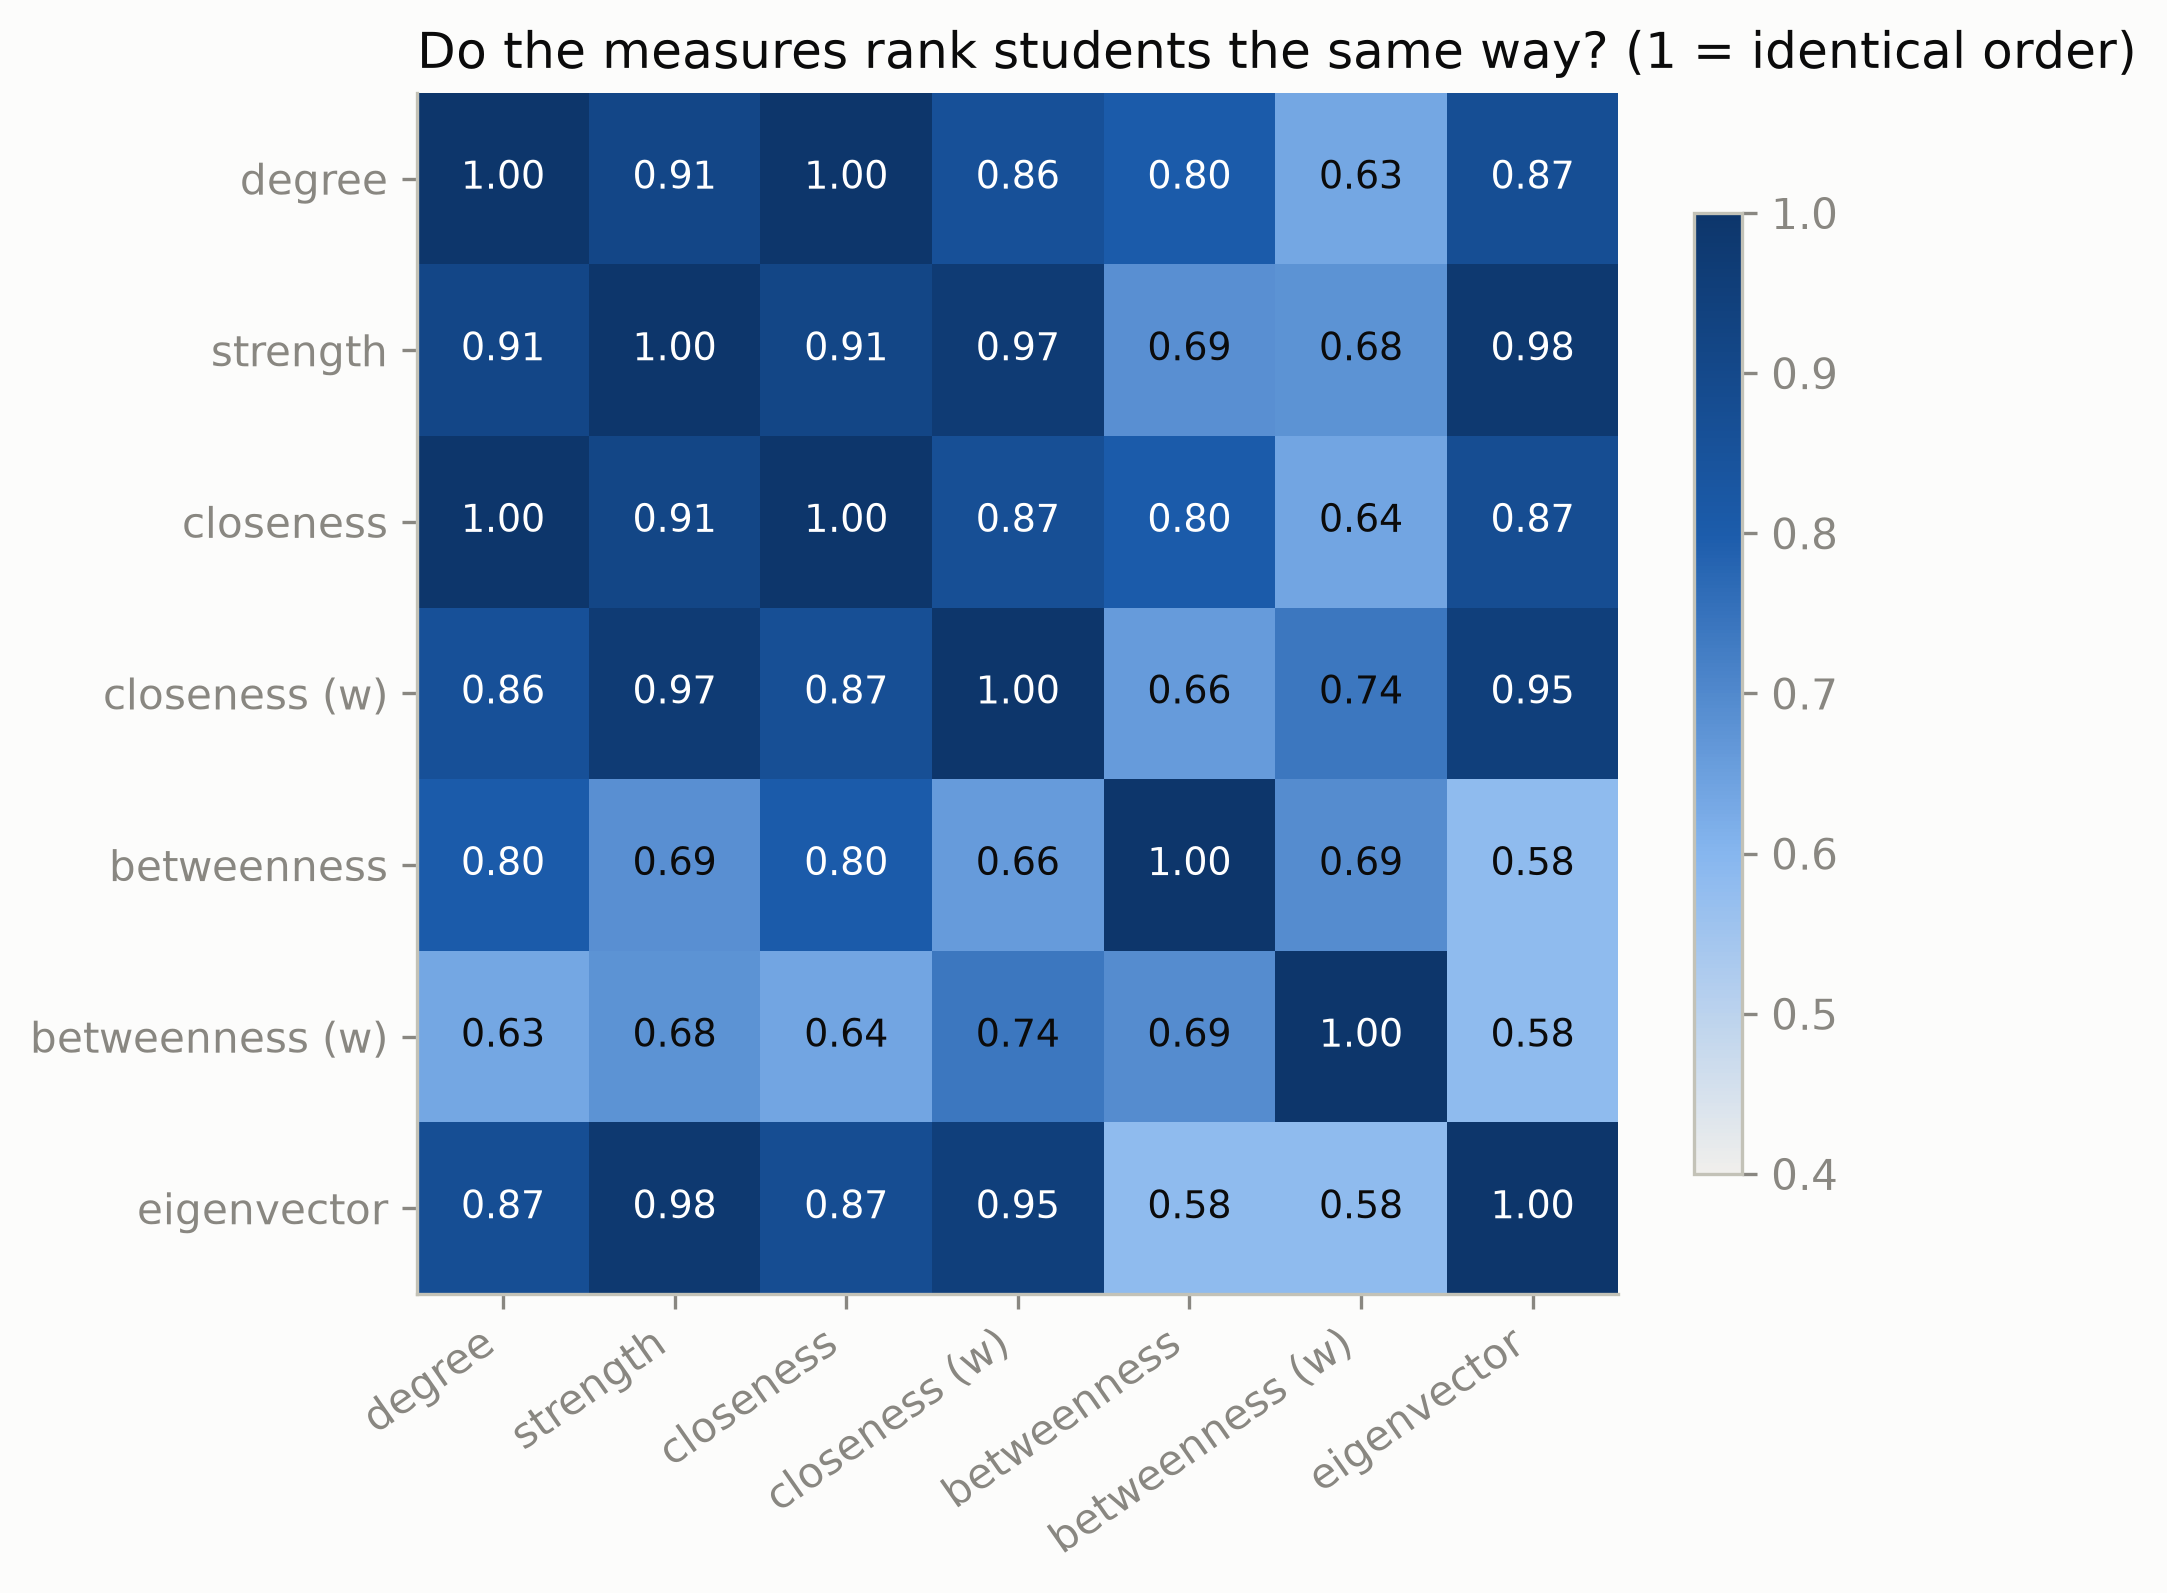
\includegraphics[width=\textwidth]{student_plots/centrality_correlations.png}
\end{minipage}\hfill
\begin{minipage}{0.45\textwidth}
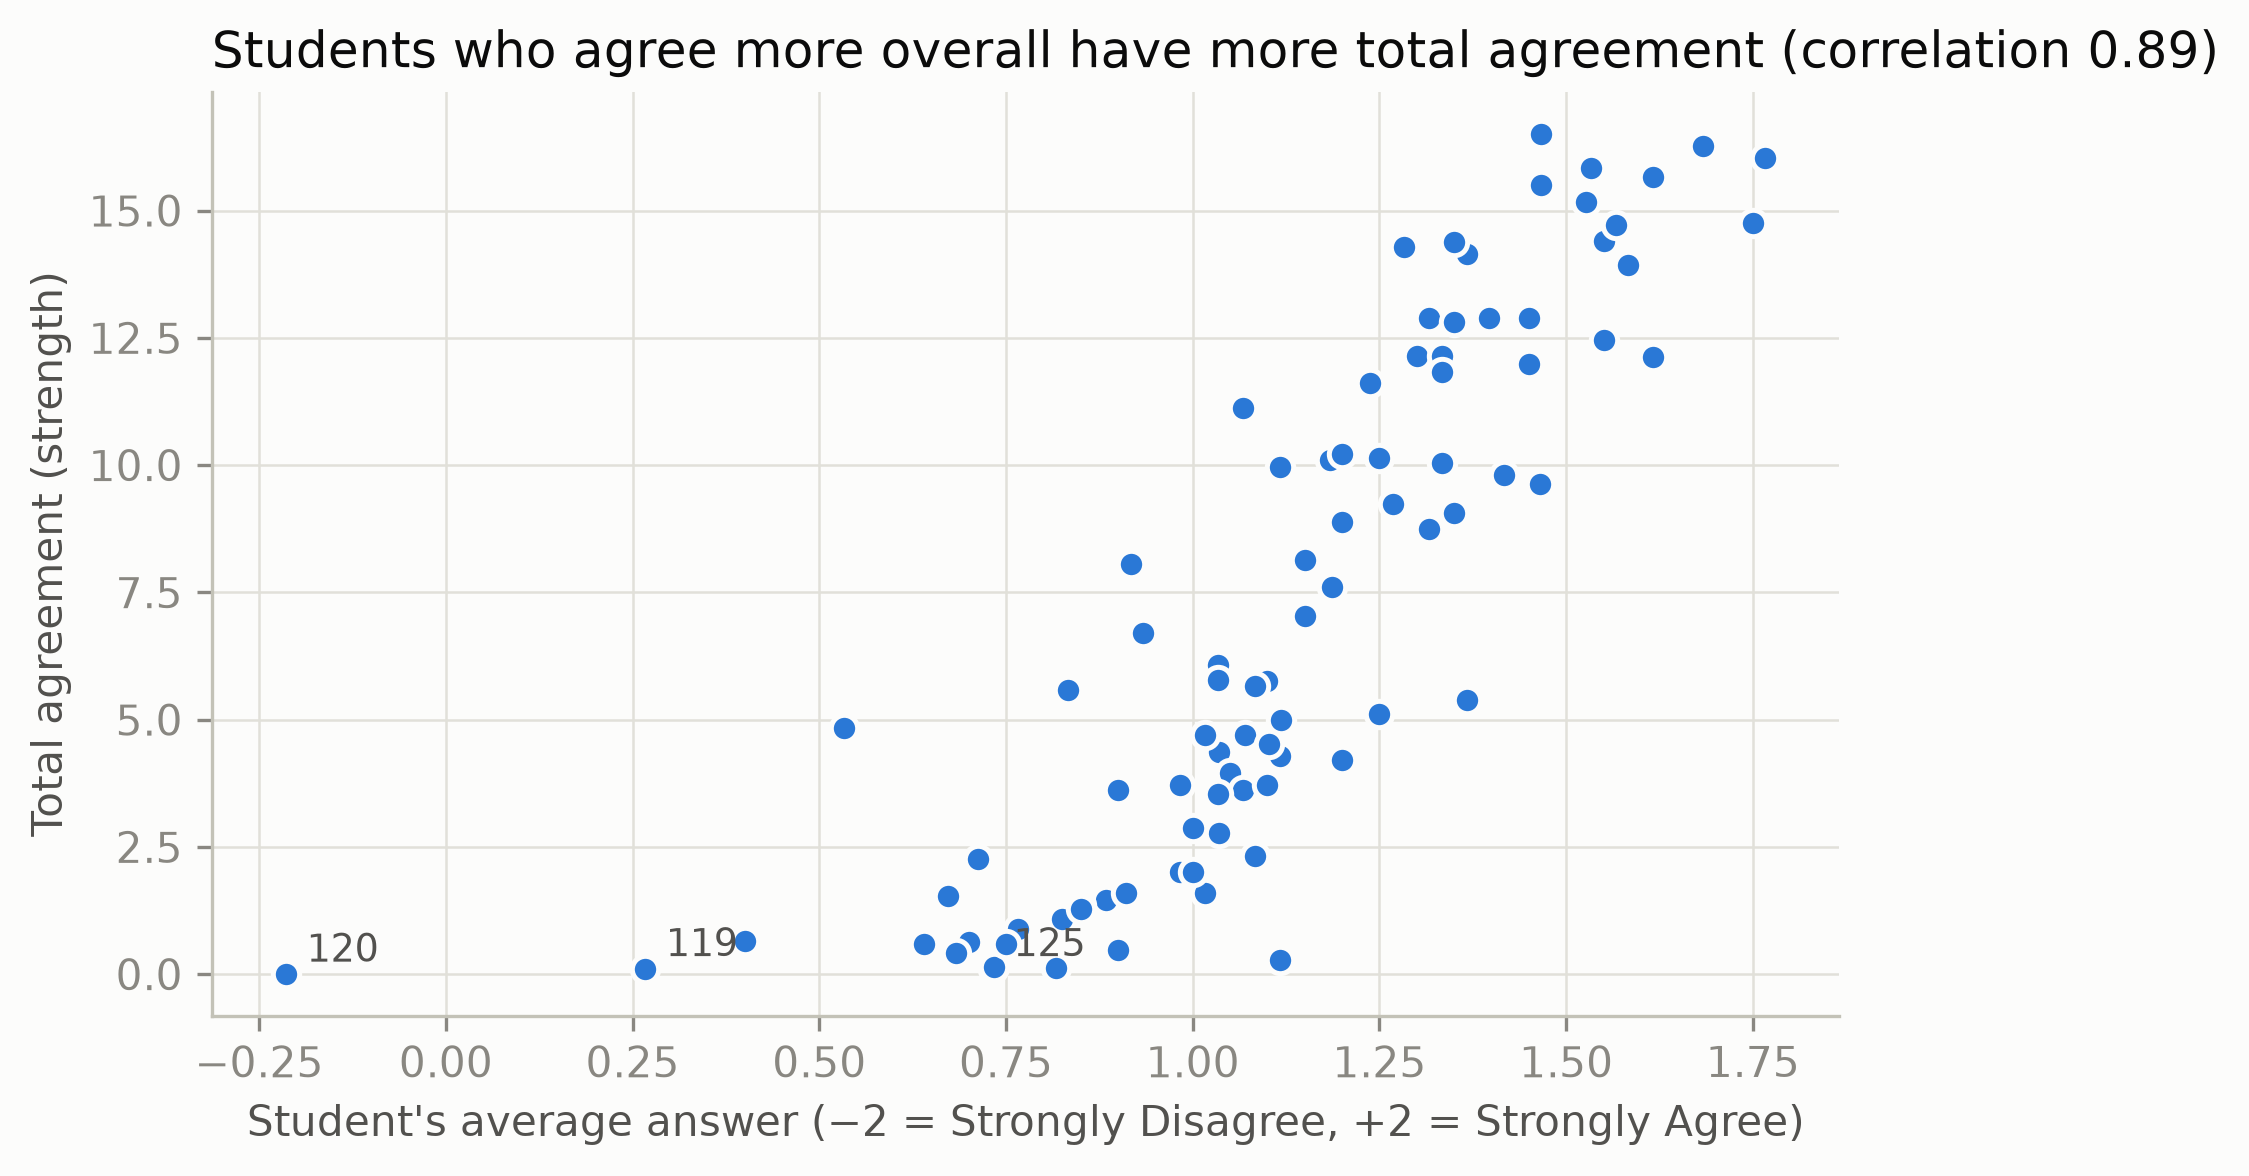
\includegraphics[width=\textwidth]{student_plots/strength_vs_mean_answer.png}
\end{minipage}
\caption{Left: how similarly the centrality measures rank the 91 students. Degree, closeness, strength and
eigenvector agree closely ($\rho \approx 0.85$--$1.00$); betweenness is the odd one out ($\rho = 0.58$--$0.80$).
Right: a student's total agreement tracks their average answer almost perfectly ($\rho = 0.89$).}
\end{figure}

\textbf{Two kinds of central student.} Strength and eigenvector centrality favour the emphatic answerers
(67, 110, 41, 114, 105), whose edges are the heaviest and mostly with each other. Degree and closeness favour a
different set (52, 99, 101, 38, 53) who mix Agree and Strongly Agree and have the \emph{most} edges. The same
emphatic core reappears in the top-2 network, so it is not an artefact of density. The periphery is stable
across every measure: 120, 125, 119, 89, 22, 63. Betweenness is led by 87 and 77, who answered only 15
questions, so that ranking is unreliable rather than meaningful.

\begin{figure}[H]
\centering
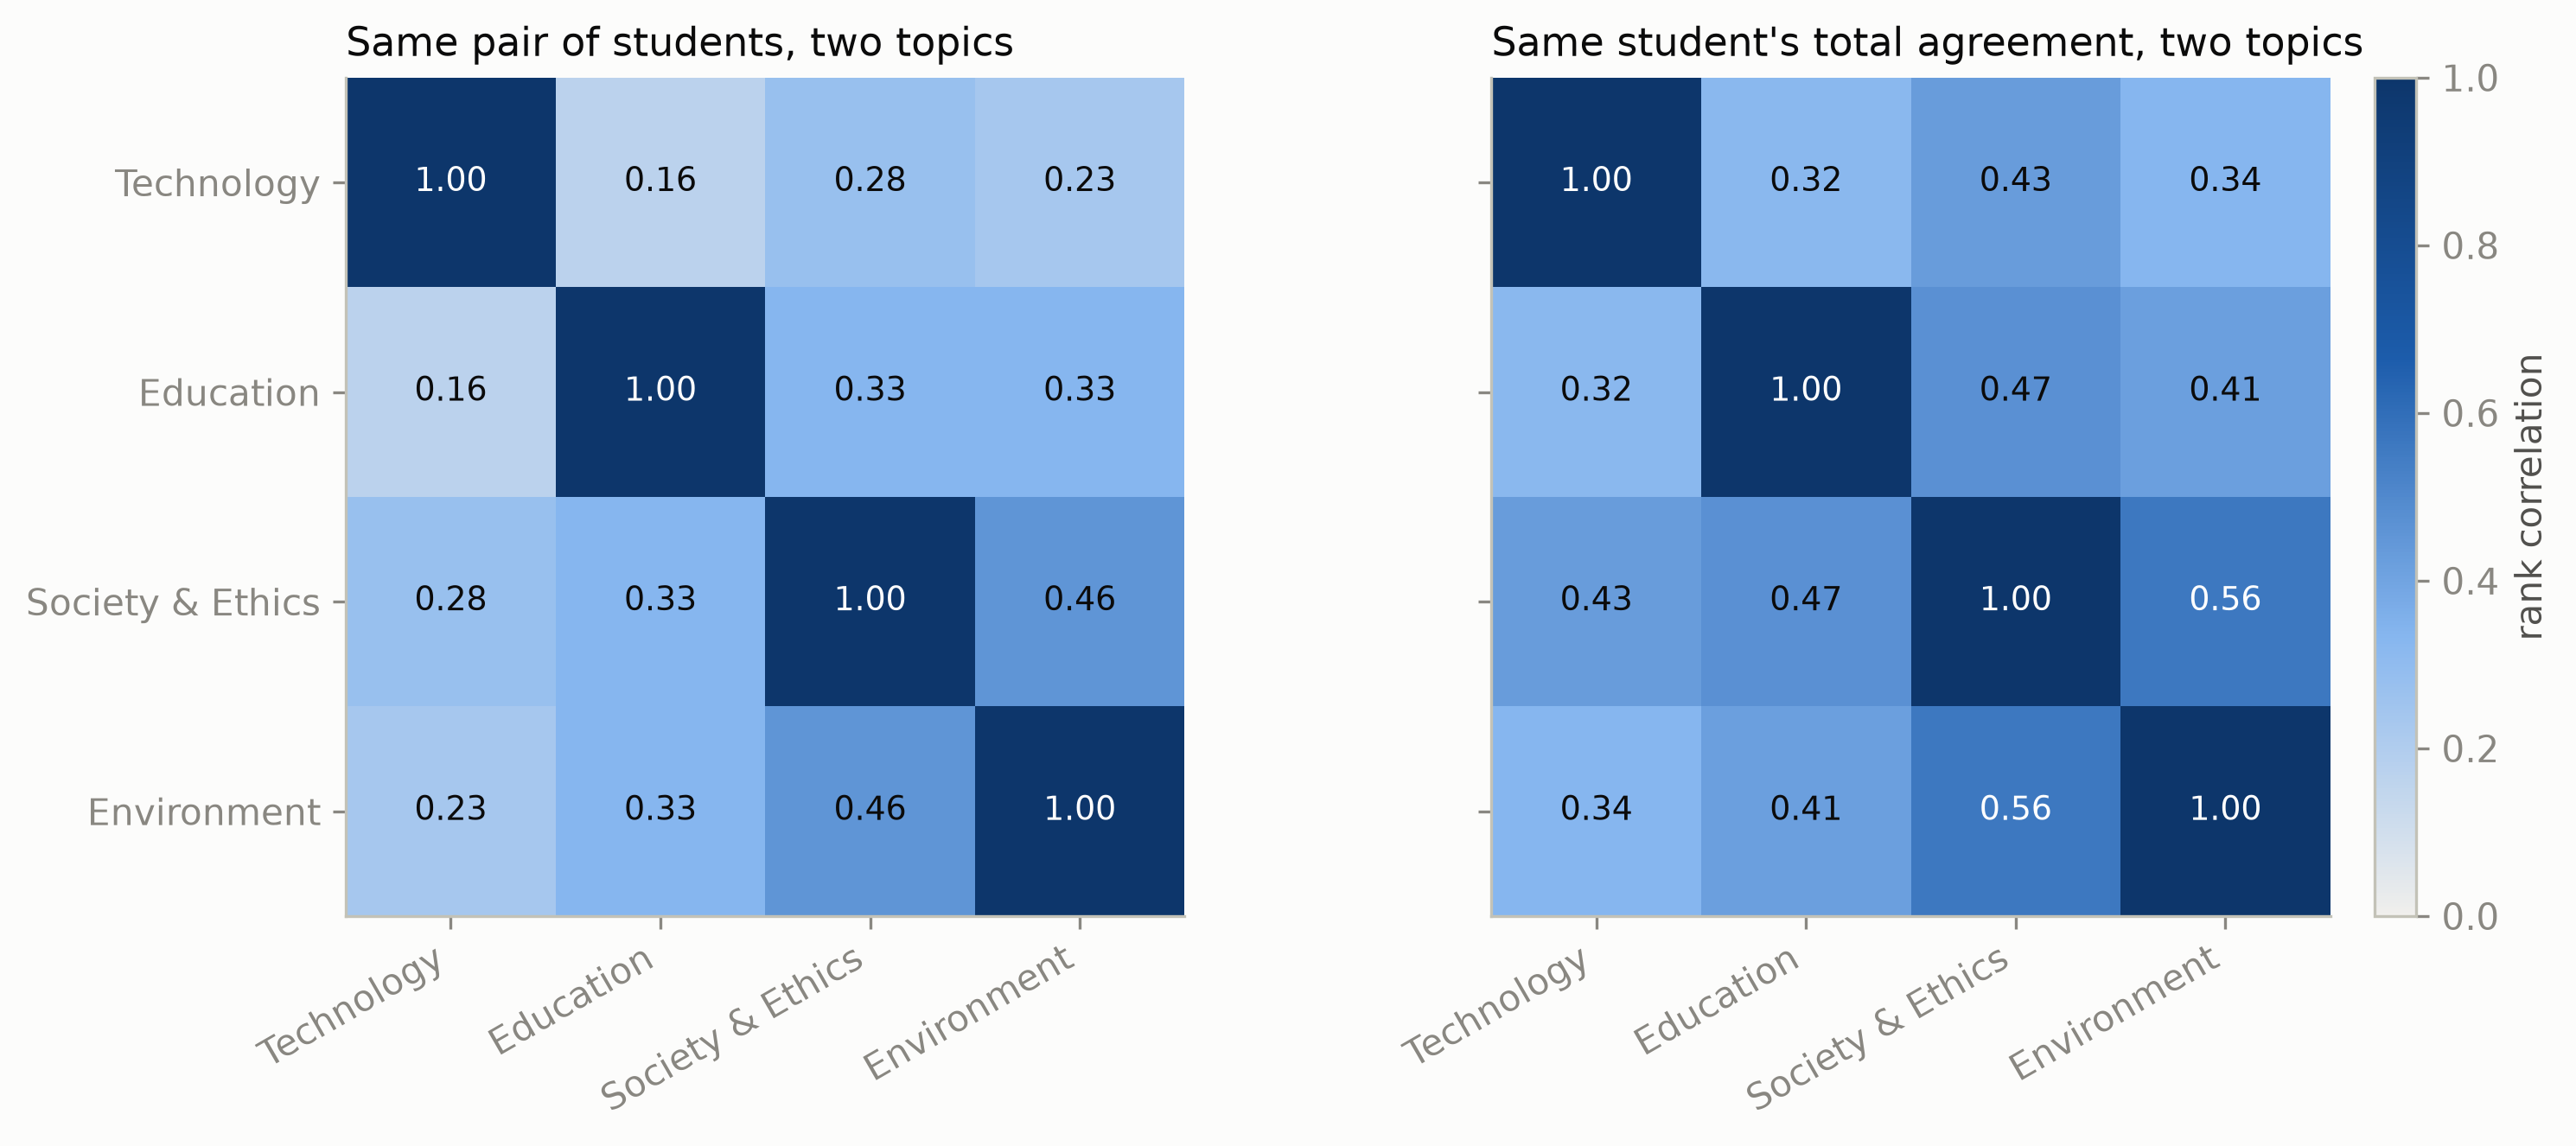
\includegraphics[width=\textwidth]{student_plots/topic_comparison.png}
\caption{One network per topic. Left: how similarly two topics score the \emph{same pair} of students. Right:
how similarly they rank the same student's total agreement. Society and Environment line students up most alike
(0.46 and 0.56); Technology and Education least (0.16). Nothing approaches 1.}
\end{figure}

Each topic alone produces a network much like the whole survey (roughly half of pairs linked, clustering
0.67--0.75), but the correlations above are all well below 1: \textbf{who a student agrees with depends on the
topic}, and agreement is not one single attitude.

\subsection{Network B: student--question extremes}

\textit{Code and figures: \texttt{Extreme Bipartite Network/main.ipynb} (Tanush Garg). Every value quoted below
was re-derived from the raw CSV for this report.}

\begin{figure}[H]
\centering
\includegraphics[width=0.9\textwidth]{bipartite_plots/bipartite_layout.png}
\caption{The bipartite extremes network: students (left) joined to the questions (right) on which they hold a
Strongly Agree or Strongly Disagree view. Question nodes are coloured by degree; the ten largest ``gravity
wells'' are labelled.}
\end{figure}

With 2{,}362 edges over a possible $89 \times 60 = 5{,}340$, the bipartite density is $0.4423$: the cohort holds
extreme views broadly rather than on a handful of pet topics. The filter retains 45.3\% of the 5{,}218 valid
responses, and the graph has exactly one connected component.

One property of this network deserves emphasis, because it governs how its results should be read:
\textbf{2{,}251 of the 2{,}362 edges (95.3\%) are Strongly Agree and only 111 are Strongly Disagree.} The
``extremes'' network is therefore very nearly a strong-\emph{agreement} network. That explains why its anchors
(E15, E11, V13) are the same statements Network~A identifies as the most consensual: an edge here records
intensity of endorsement, not opposition, so questions approaching unanimity dominate. Section by section, the
mean question degree is highest for Environment (44.5) and Society (41.6) and \emph{lowest} for Technology
(33.9), so the extreme opinion in this cohort is concentrated in environmental and civic statements rather than
technological ones --- the mirror image of Network~A's finding that the most divisive questions are largely
technological.

\begin{figure}[H]
\centering
\includegraphics[width=0.78\textwidth]{bipartite_plots/degree_distribution_linear.png}
\caption{Linear-binned degree distribution of the 60 question nodes with a fitted normal curve
($\mu = 39.37$, $\sigma = 12.16$; range 11--64). The peaked, bounded shape rules out the monotonic decay of a
power law.}
\end{figure}

\begin{figure}[H]
\centering
\includegraphics[width=\textwidth]{bipartite_plots/degree_distribution_loglog.png}
\caption{Log-log degree distribution with logarithmic binning (left) and the complementary CDF (right). The
best-fit exponent $\hat{\gamma} = 0.750$ lies far outside the $2 < \gamma < 3$ band required of a scale-free
network, and both curves bend rather than run straight.}
\end{figure}

The distribution is not Poisson either: the dispersion index
$\mathrm{Var}(k)/\langle k \rangle = 147.9/39.4 \approx 3.75$ is nearly four times the ER expectation of 1. The
extremes network is \textbf{bounded but overdispersed} --- no mega-hubs, yet some questions attract far more
intensity than chance allows.

\subsection{Network C: question--question projection}

\textit{Code and figures: \texttt{Extreme Bipartite Network/main.ipynb} (Tanush Garg).}

\begin{figure}[H]
\centering
\includegraphics[width=0.85\textwidth]{bipartite_plots/projected_network.png}
\caption{The question--question projection. Every pair of questions is joined, i.e.\ the unweighted projection is
the complete graph $K_{60}$ (1{,}770 edges, density 1.0, clustering 1.0, average path length 1.0). Colour marks
the four survey domains.}
\end{figure}

Completeness is itself the finding: \textbf{for every pair of questions there is at least one student holding
extreme views on both}, so extreme opinion in this cohort is not organised into subject-specific silos. It also
means unweighted centrality is uniform --- every question has degree 59 --- which is why the weighted projection
$G_Q^W$ carries the analysis. Three measures are used on it, the same ones defined in Section~5.1, now applied to questions: \textbf{strength} $C_S(v) = \sum_{u} w_{vu}$, the total number of shared
extreme views, normalised by the largest such total; \textbf{weighted betweenness}, computed with edge lengths
$d_{ij} = 1/w_{ij}$ so that heavily shared pairs count as close together; and \textbf{weighted eigenvector}
centrality, $C_E(v) = \lambda^{-1} \sum_u w_{vu} C_E(u)$, which rewards questions co-held with other central
questions.

\begin{figure}[H]
\centering
\includegraphics[width=\textwidth]{bipartite_plots/centrality_bars.png}
\caption{Strength, weighted betweenness and weighted eigenvector centrality on $G_Q^W$. Strength and
eigenvector decay gradually; betweenness is sharply skewed, collapsing after the top five questions.}
\end{figure}

\begin{figure}[H]
\centering
\includegraphics[width=0.55\textwidth]{bipartite_plots/centrality_heatmap.png}
\caption{All 60 questions across the three weighted measures. The hot rows are the questions that act as
ideological anchors.}
\end{figure}

\begin{center}
\begin{tabular}{l p{8.6cm} c c}
\toprule
\textbf{ID} & \textbf{Statement} & \textbf{Strength} & \textbf{Eigenvector} \\
\midrule
E15 & Continuous learning and skill development are essential throughout one's career & 1.000 & 0.186 \\
E11 & University curricula should be updated more frequently for emerging technologies & 0.988 & 0.184 \\
V13 & Companies should be accountable for their environmental impacts & 0.979 & 0.183 \\
V09 & Products should be designed for reuse, repair and recycling & 0.961 & 0.180 \\
S05 & Individuals should control how their personal data are collected and used & 0.917 & 0.172 \\
S11 & People should be free to express differing opinions (absent harm) & 0.901 & 0.168 \\
V14 & International cooperation is necessary for environmental challenges & 0.883 & 0.166 \\
E10 & Universities should prioritise innovation over rote learning & 0.875 & 0.164 \\
\bottomrule
\end{tabular}
\captionof{table}{The strongest ideological anchors in $G_Q^W$. Weighted betweenness ranks the same three
questions first (E15 0.084, E11 0.036, V13 0.025) before collapsing towards zero.}
\end{center}

The \textbf{Molloy--Reed criterion} gives the condition for a giant component to exist in a network with a given
degree sequence: $\kappa = \langle k^2 \rangle / \langle k \rangle > 2$, where $\langle k \rangle$ is the mean
degree and $\langle k^2 \rangle$ the mean squared degree. Here every question has degree 59, so
$\langle k \rangle = 59$, $\langle k^2 \rangle = 3{,}481$ and $\kappa = 59$ --- the largest value a 60-node graph
can reach, and far above the threshold of 2.

\begin{figure}[H]
\centering
\includegraphics[width=\textwidth]{bipartite_plots/molloy_reed.png}
\caption{Molloy--Reed criterion on the unweighted projection. Every node has degree 59, giving
$\kappa = \langle k^2 \rangle / \langle k \rangle = 59 \gg 2$: the giant component is guaranteed, by the widest
possible margin for a 60-node graph.}
\end{figure}

\begin{figure}[H]
\centering
\includegraphics[width=\textwidth]{bipartite_plots/robustness_simulation.png}
\caption{Robustness of the unweighted projection under targeted attack (highest degree first) and random
failure. In $K_{60}$ the two are mathematically indistinguishable and the giant component holds at 1.0 until the
graph is nearly exhausted, because removing a node from a complete graph leaves a complete graph.}
\end{figure}

\subsection{Network D: question--question correlation}

\textit{Code and figures: \texttt{Question Network/question\_network.ipynb} (Amish Goyal). Every value quoted
below was re-derived from the raw CSV for this report.}

At the $\rho > 0.35$ cutoff the network keeps \textbf{188 of the 1{,}770 possible edges} (density 0.106, average
degree 6.27). It is not one connected whole: 47 questions form a giant component, and \textbf{13 questions are
left isolated}, correlating strongly with nothing at all. This is the first of the four networks that
fragments, and the fragmentation is the finding.

\begin{figure}[H]
\centering
\includegraphics[width=0.86\textwidth]{question_plots/network_graph.png}
\caption{The question--question correlation network. Node colour marks the survey section (blue Technology,
orange Education, green Society \& Ethics, purple Environment), node size is eigenvector centrality and edge
width is $\rho$. Sections mix, but the environmental block stands out as a dense, almost unmixed region.}
\end{figure}

\begin{figure}[H]
\centering
\includegraphics[width=0.94\textwidth]{question_plots/correlation_heatmap.png}
\caption{All $60 \times 60$ Spearman correlations, with the statements grouped by section (in the order E, S, T,
V). The strongest block by far is Environment, in the lower right: environmental statements move together.
The Technology block is visibly paler, so technology opinions co-vary far less. The two red rows near the top
are E02 (written exams measure knowledge) and E03 (compulsory attendance), which correlate \emph{negatively}
with much of the survey and therefore join nothing at a positive cutoff.}
\end{figure}

\begin{figure}[H]
\centering
\includegraphics[width=0.94\textwidth]{question_plots/centrality_rankings.png}
\caption{Top ten statements by eigenvector centrality (ideological anchors, left) and by weighted betweenness
(cross-domain bridges, right).}
\end{figure}

\begin{center}
\small
\begin{tabular}{llcc p{6.4cm}}
\toprule
\textbf{Role} & \textbf{ID} & \textbf{Section} & \textbf{Score} & \textbf{Statement} \\
\midrule
Anchor & V07 & V & 0.309 & Protecting biodiversity is essential for long-term well-being \\
(eigenvector) & S09 & S & 0.295 & Universities should promote an inclusive environment \\
 & V08 & V & 0.285 & Universities should adopt sustainable campus practices \\
 & V10 & V & 0.269 & Consumers should consider environmental impact when purchasing \\
 & V12 & V & 0.264 & Sustainability should be integrated into higher education \\
\midrule
Bridge & S09 & S & 0.099 & Universities should promote an inclusive environment \\
(betweenness) & S13 & S & 0.098 & Critical evaluation of online information should be taught \\
 & T12 & T & 0.074 & Governments should introduce stricter AI regulation \\
 & S14 & S & 0.061 & Leaders should prioritise ethical decision-making \\
 & S10 & S & 0.055 & Scientific evidence should inform public policy \\
\bottomrule
\end{tabular}
\captionof{table}{Anchors and bridges in Network~D. Eight of the top ten anchors are environmental statements.}
\end{center}

\begin{figure}[H]
\centering
\includegraphics[width=0.8\textwidth]{question_plots/centrality_landscape.png}
\caption{Eigenvector against betweenness centrality. Most statements sit near the origin; S09 is the rare
statement that is both an anchor and the network's primary bridge, while S13 and T12 bridge without being
anchors.}
\end{figure}

\textbf{Reading Network D.} Three results stand out.

\begin{itemize}[nosep]
  \item \textbf{The belief core is environmental and ethical.} Eight of the ten highest eigenvector scores are
  Environment statements, interlocked with the ethics items S09 and S14. Agreement on biodiversity, sustainable
  campuses and responsible consumption moves as one block.
  \item \textbf{The bridges are the contested interfaces.} S09 (inclusion), S13 (digital literacy) and T12 (AI
  regulation) sit between clusters. They are where technology opinion connects to educational and civic
  opinion, and therefore where a change of mind would propagate furthest.
  \item \textbf{Beliefs do not follow the syllabus.} Louvain finds six organic modules, and section
  assortativity is only $r = 0.304$: sections matter, but students do not compartmentalise by them. Two modules
  are genuinely mixed --- AI governance (T03, T10, T12, T13 with S05) and educational modernisation (education
  items with T01, T02, T06, S07, S11, V02) --- while ecology forms an almost purely environmental module.
\end{itemize}

\section{Results and Discussion}

\textbf{1. The class agrees far more than it disagrees, and that shapes every network.} Four in five answers are
on the agree side. In Network~A this makes raw agreement useless as a similarity measure --- it links everyone
to everyone --- and forces the chance correction. In Network~B the same fact appears as a bipartite density of
0.44, and in Network~C as a complete projection. Only Network~D, which measures co-movement rather than
agreement, escapes it: at $\rho > 0.35$ just 10.6\% of question pairs survive.

\textbf{2. Intensity and alignment pick out different questions, and the contrast is the most informative
result in the project.} Network~A finds E15, V13, S05, E11 and V09 to be the \emph{most consensual} questions,
the ones where a matching answer says almost nothing about a pair. Network~C finds exactly those questions to be
the strongest ideological anchors, because a near-unanimous Strongly Agree makes a question both the biggest
gravity well for extreme opinion and the least informative for telling students apart. Network~D then ranks that same E15 \textbf{26th} of the 47 questions in its
giant component: with almost no variance left, a question everyone endorses cannot correlate with anything. Its anchors are instead V07, S09, V08, V10 and V12 --- statements that people genuinely vary on, and
vary on \emph{together}. Read as a set: E15 is what the class believes, V07 and S09 are what its beliefs are
organised around.

\textbf{3. The questions that split the class are the ones that belong to no structure at all.} Network~A ranks
statements by chance agreement $E_q$; its five most divisive are E02 (written exams measure knowledge,
$E_q = 0.58$), T08 (AI diagnosis, 0.58), E04 (online learning, 0.63), T09 (autonomous vehicles, 0.64) and E13
(research over infrastructure, 0.72). Network~D, built by an entirely different route, leaves 13 questions
isolated at $\rho > 0.35$: E02, E03, E04, E08, E09, E13, S08, T04, T05, T08, T09, T14 and T15. \textbf{All five
of Network~A's most divisive statements are in that list.} One method compares pairs of students, the other
pairs of questions, and they agree: where this class divides, it divides idiosyncratically, without lining up
along any shared axis.

\textbf{4. Nothing fragments except where we force it to.} Network~A's largest component erodes one student at
a time under thresholding, with no percolation-style collapse; Network~B has a single connected component;
Network~C is complete, with $\kappa = 59 \gg 2$ and no distinction between random failure and targeted attack.
Network~D fragments only because a cutoff is imposed, and what falls out --- the 13 isolates --- is precisely the
contested material. The cohort has no echo chambers and no topic silos.

\textbf{5. Structure is small-world and broad, but never scale-free.} Network~A is clustered well above random
(6$\times$ in its sparse version) at random-like distances, $\sigma = 1.46$ and $5.66$. Network~B's question
degrees are overdispersed (dispersion index 3.75) but bounded, with $\hat{\gamma} = 0.750$, nowhere near the
scale-free band. Both are broader than an ER graph and far from a power law --- unsurprising at $N = 91$ and
$N = 60$, and worth stating as a limit rather than a discovery.

\textbf{6. Centrality in Network A largely measures agreeableness; in Network D it measures alignment.} A
student's total agreement tracks their average answer at $\rho = 0.89$, and the emphatic answerers hold the
heaviest edges, so being ``central'' among students mostly means agreeing readily. Among questions, centrality
means something sharper: S09 is simultaneously an anchor and the primary bridge, so inclusion is both a core
commitment and the hinge connecting educational, civic and environmental opinion.

\textbf{7. Topic matters, and the two halves of the project agree on how.} Network~A finds Society and
Environment line students up most alike (pair scores 0.46, strengths 0.56) and Technology and Education least
(0.16). Network~D finds the same asymmetry from the question side: ecology forms an almost unmixed module and
the environmental block is the brightest region of the correlation heatmap, while technology items scatter into
AI-governance and educational-modernisation modules. Section assortativity of $r = 0.304$ says the survey's own
four sections are a weak guide to how these students actually think.

\textbf{Limitations.} The cohort is small (91 usable responses), so degree-distribution claims are bounded by
$N$; three respondents in Networks~B and~C answered only 15 of the 60 questions, which understates their degree
there and inflates their betweenness in Network~A; Network~D's structure depends on one free parameter, the
$\rho > 0.35$ cutoff, which sets how many questions end up isolated; and a Likert survey cannot separate genuine
conviction from a habit of reaching for the end of a scale, so ``emphatic'' should be read as a response
pattern, not a personality.

\section{Individual Contribution}

\begin{center}
\begin{tabular}{p{3.2cm} p{11.5cm}}
\toprule
\textbf{Member} & \textbf{Contribution} \\
\midrule
\textbf{Mayank Kar} &
Network~A (student--student), and this combined report. Shared cleaning and encoding module \texttt{clean.py} used by the whole team;
the simple and chance-adjusted agreement scores; the sparsification experiments (global threshold sweep and the
top-2 construction); the structural measurements against ER graphs, including clustering, path lengths,
efficiency, small-world $\sigma$ and assortativity; all five centrality measures and their rank comparison; the
per-topic networks; \texttt{student\_network.ipynb} and the eight figures in \texttt{student\_plots/}. \\
\addlinespace
\textbf{Tanush Garg} &
Networks~B and~C (student--question bipartite and its question--question projection). The extremes filter and
long-format edge list; construction and validation of the bipartite graph; bipartite topology (density,
components, isolated respondents); question-node degree distribution with linear and logarithmic binning, the
power-law fit and the dispersion analysis; the projection onto the question set and the weighted projection
$G_Q^W$; strength, weighted betweenness and weighted eigenvector centrality on it; the Molloy--Reed evaluation
and the robustness simulation; \texttt{main.ipynb}, the eight figures in \texttt{extreme\_plots/} and the interactive
D3 visualisers. \\
\addlinespace
\textbf{Amish Goyal} &
Network~D (question--question correlation). Pairwise Spearman correlation across all 1{,}770 question pairs on
the shared cleaned data; the thresholded graph at $\rho > 0.35$ with affinity weights and inverse-$\rho$
distances; weighted eigenvector and metric betweenness centrality; Louvain community detection and the
interpretation of the six modules; the section assortativity coefficient and identification of the isolated
questions; \texttt{question\_network.ipynb}, the four figures in \texttt{Question Network/}, the repository's initial
setup and its later reorganisation into per-network folders, and the project landing page
\texttt{index.html}. \\
\bottomrule
\end{tabular}
\end{center}

\end{document}
